\chapter{Results}
\label{chap:results}

\section{Interface}
\todo{write something about performance. when does mesh become too heavy for VR rendering}
As mentioned in the previous chapter, SketchMeshVR does not make use of any menus and instead solely relies on different combinations of button presses to differentiate between the multiple available modeling actions. This does require more effort from the user in order to keep track of the selected editing modes, but at the same time keeps the interface cleaner. In order to guide the user when drawing strokes, SketchMeshVR provides visual feedback on the positions that will be used to create a stroke. In case of the drawing and curve deformation modes this means that the user sees the position controller and in case of all other modes the user will see the position controller plus a ray shooting from it (the ray ends at any intersections it has with the scene). Figures~\ref{fig:interface}(a) and (b) show what this looks like.

\begin{figure}[!h]
    \centering
    \setlength{\tabcolsep}{0.0130\linewidth}
    \begin{tabular}{@{}cc@{}}
    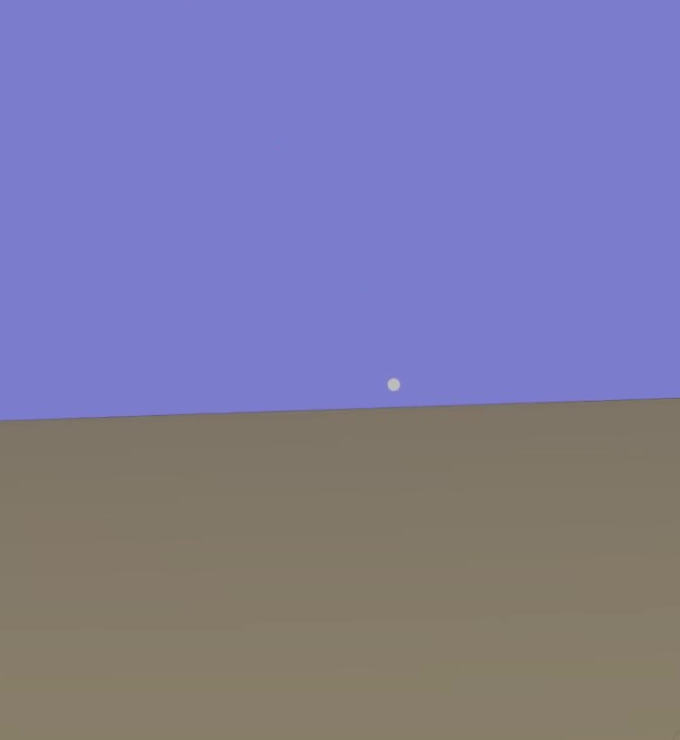
\includegraphics[width=0.3\linewidth]{figures/interface_point}&
  	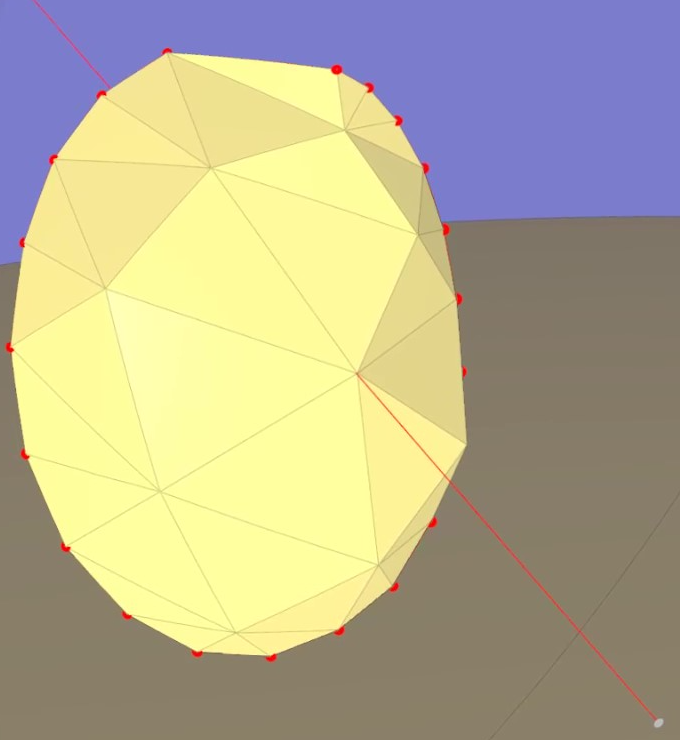
\includegraphics[width=0.3\linewidth]{figures/interface_ray}\\
    (a)&(b)\\
    \end{tabular}
    \caption[SketchMeshVR interface]{SketchMeshVR interface.
    	  \textup{(a)} Controller reference point that is displayed in drawing and deformation mode.
			  \textup{(b)} Controller and ray reference that are displayed in all other editing modes. 
      \label{fig:interface}}
\end{figure}
 
\section{User review}
Our program has been tested by users that had none to little prior experience with 3D modeling and also had none to little experience with VR. The test users were requested to first try and recreate one of the example models from Figures~\ref{fig:recreate_dolphin} or~\ref{fig:recreate_teddy} using SketchMeshVR and then to recreate the same model in the non-VR version of the software. Users reported that although it took some initial effort to get acquainted with the controls, it was very easy to learn how to use SketchMeshVR. They also reported that the immersive nature of VR made the interaction with the created mesh much more impressive compared to the non-VR SketchMesh. Although the users had experience with creating the given models when they modeled them in non-VR, it took them longer to recreate the model than when using SketchMeshVR. Figures~\ref{fig:recreate_teddy} and~\ref{fig:recreate_dolphin} show side-by-side comparisons of the example models that were given to the test users, and the models that they created in both the non-VR and VR versions of our software. As you can see, the users managed to create models that were similar to the example models that were provided to them. While creating these models, users did not experience any fatigue in their hands. When using the software for a prolonged period though (15 minutes or more), users started to feel tiredness in their arms due to the relatively large body movement as compared to mouse movement. Users did not experience fatigue from the VR rendering while using the application and reported that they found the rendering to be very smooth. However, after prolonged wear of the headset some users reported an uncomfortable feeling from the pressure on the face because of the weight of the Oculus Rift headset. 


\begin{figure}[!h]
    \centering
    \setlength{\tabcolsep}{0.0130\linewidth}
    \begin{tabular}{@{}ccc@{}}
    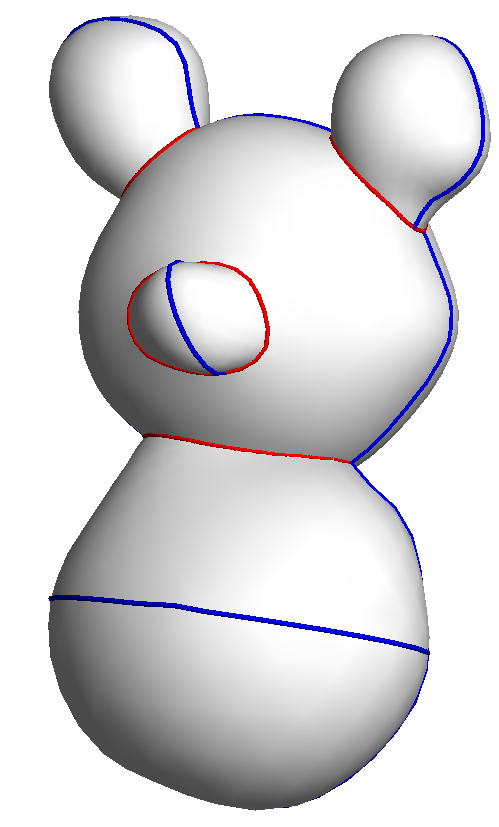
\includegraphics[width=0.3\linewidth]{figures/example_model_figure}&
  	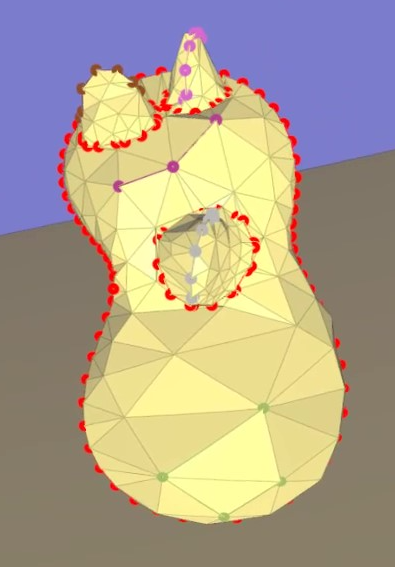
\includegraphics[width=0.3\linewidth]{figures/results_teddy_model1}&
  	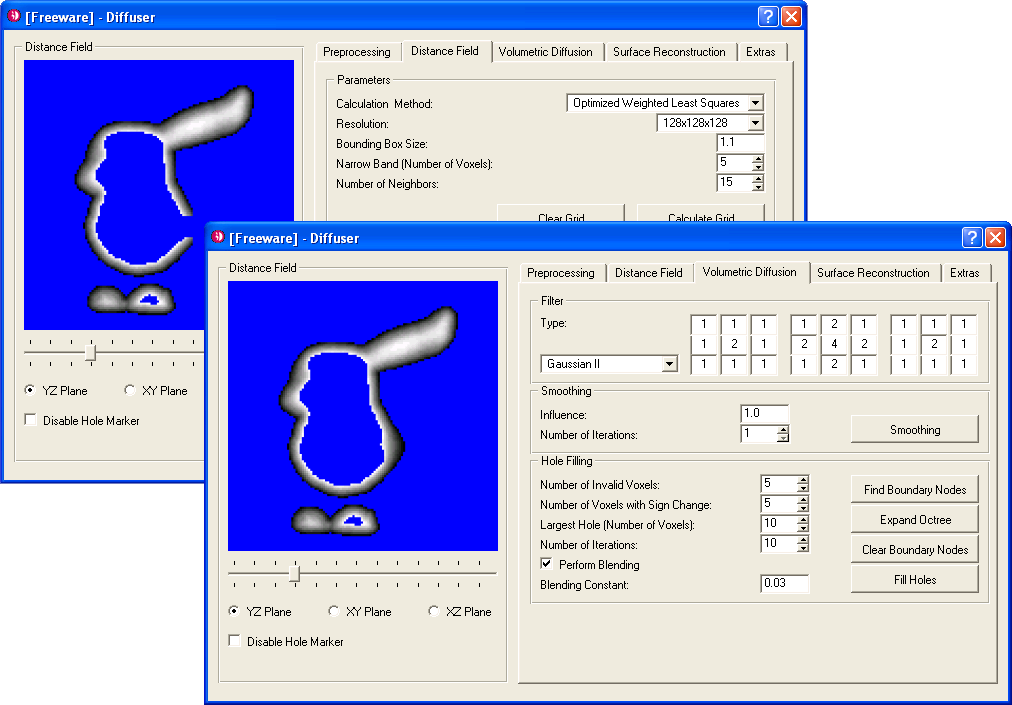
\includegraphics[width=0.3\linewidth]{figures/voldiff_ui}\\

    (a)&(b)&(c)\\
    \end{tabular}
    \caption[SketchMeshVR simplified teddy bear model]{SketchMeshVR recreating models.
    	  \textup{(a)} Example mesh of a simplified teddy bear.
	  \textup{(b)} Resulting recreated model made in VR (took 5 minutes to complete).
	  \textup{(c)} Resulting recreated model made in non-VR (took 8 minutes to complete).
      \label{fig:recreate_teddy}}
\end{figure}


\begin{figure}[!h]
    \centering
    \setlength{\tabcolsep}{0.0130\linewidth}
    \begin{tabular}{@{}ccc@{}}
    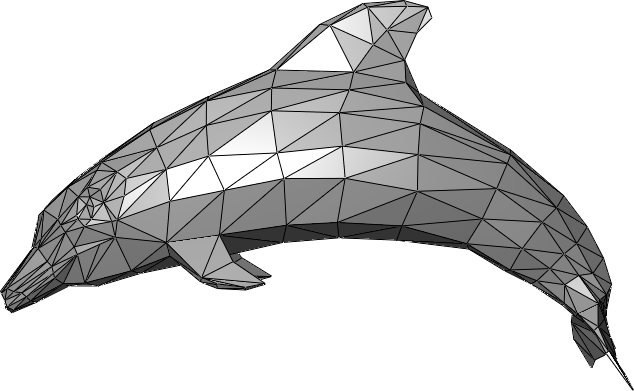
\includegraphics[width=0.3\linewidth]{figures/example_model_dolphin}&
  	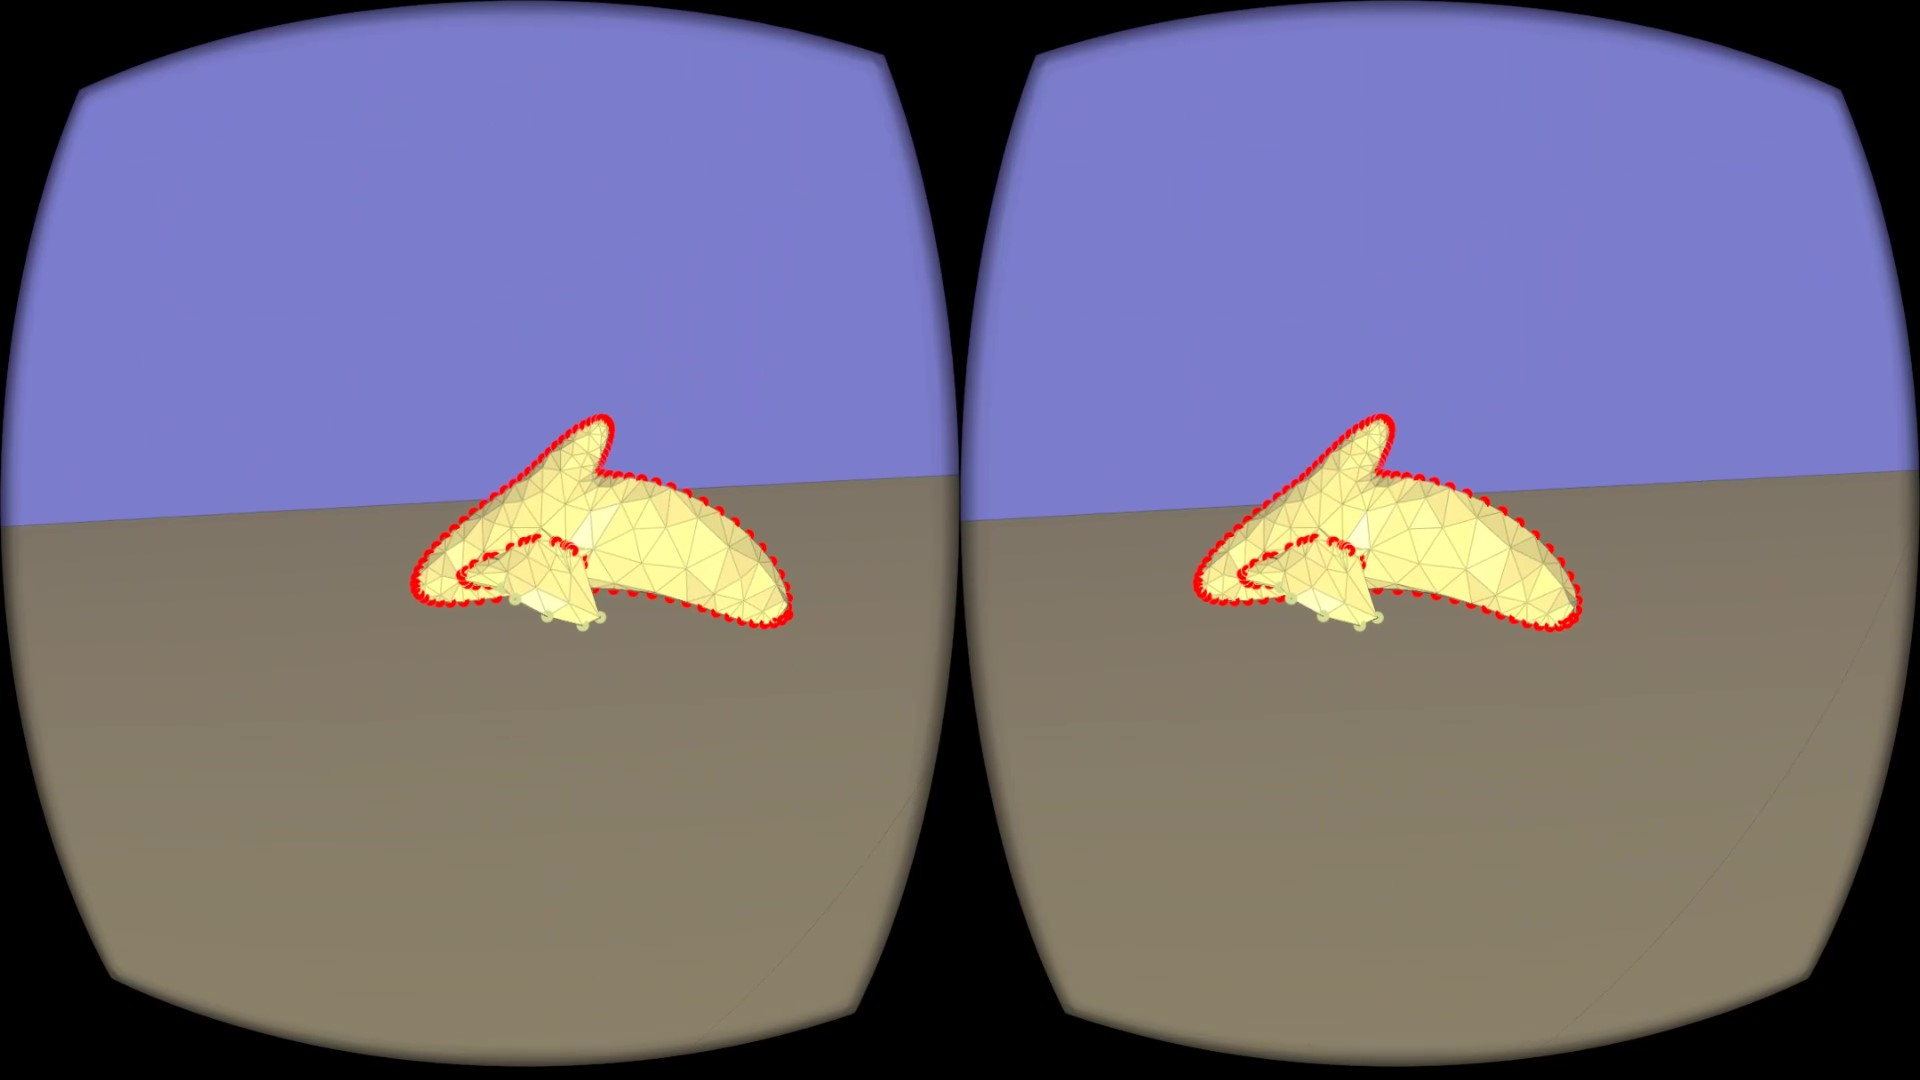
\includegraphics[width=0.3\linewidth]{figures/results_dolphin_model}&
  	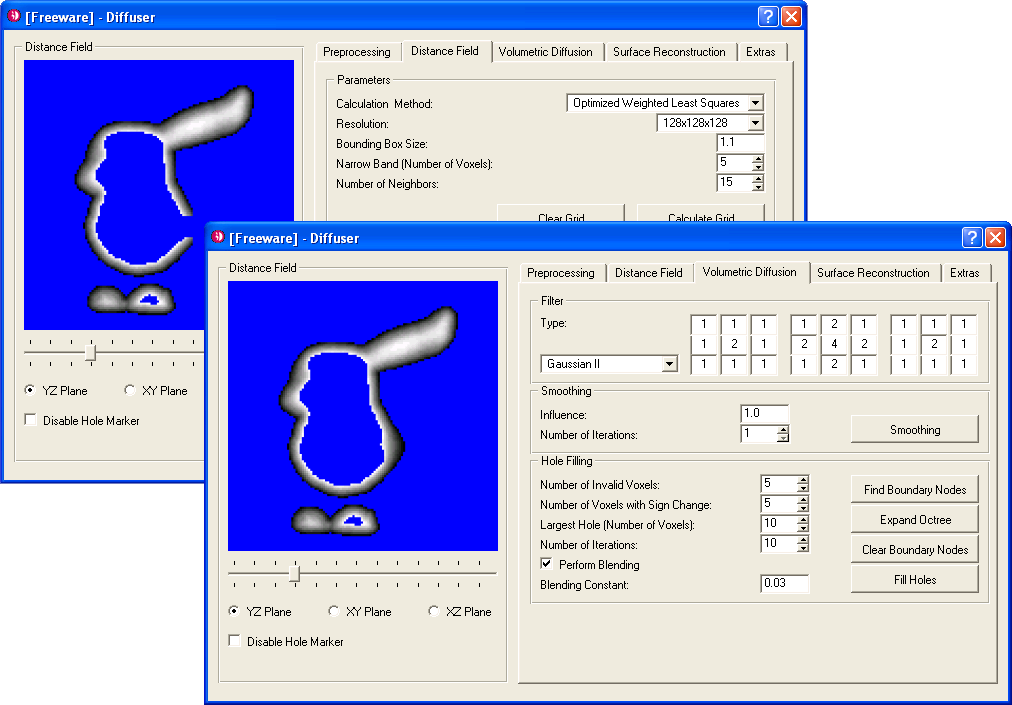
\includegraphics[width=0.3\linewidth]{figures/voldiff_ui}\\

    (a)&(b)&(c)\\
    \end{tabular}
    \caption[SketchMeshVR dolphin model]{SketchMeshVR recreating models.
    	  \textup{(a)} Example simplified mesh of a dolphin.
	  \textup{(b)} Resulting recreated model made in VR (took 4 minutes to complete).
	  \textup{(c)} Resulting recreated model made in non-VR (took 6 minutes to complete).
      \label{fig:recreate_dolphin}}
\end{figure}
\todo{Mention size of meshes and when slow-down will be noticeable}


Also users reported that they found the modeling to be considerably more effortless in VR, as it requires less intermediate navigation of the mesh between modeling steps (for example before drawing the extrusion silhouette or making a diagonal cut there is no need to rotate the mesh in VR). However they did also remark that actions that required larger precision, such as curve deformation on curves that are close to eachother, were easier to perform with the mouse than in VR.
Additionally users noted that the possibility to define strokes in an additional dimension provides added artistic freedom, for example when defining the extrusion silhouette the user can now draw a S-shaped curve and choose where it will be positioned inside the extrusion base, whereas the non-VR mode forces extrusion silhouettes to be straight lines. 
